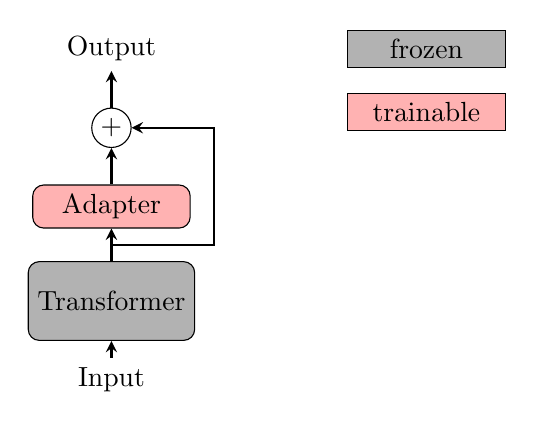
\begin{tikzpicture}[node distance=1cm]


    \tikzstyle{transformers} = [rectangle, minimum width=2cm ,text centered, draw=black, fill=black!30]
    \tikzstyle{adapter} = [rectangle, minimum width=2cm , text centered, draw=black, fill=red!30]
    \tikzstyle{arrow} = [thick,->,>=stealth]
    
    \tikzstyle{sum} = [circle, draw, minimum size=0.5cm, node distance=1cm, inner sep=0pt]
    
    % Define nodes
    \node (output)[]{Output};
    \node (plus)[sum, below of=output]{+};
    \node (adapter)[adapter,rounded corners, below of=plus]{Adapter};
    \node (transformer)[transformers,rounded corners, below of = adapter, minimum height=1cm, yshift=-0.2cm]{Transformer};
    \node (input)[below of = transformer]{Input};

    % vertical arrows
    \draw[arrow] (input) -- (transformer);
    \draw[arrow] (transformer) -- (adapter);
    \draw[arrow] (adapter) -- (plus);
    \draw[arrow] (plus) -- (output);

    % side arrow
    \draw[arrow] ([yshift=0.2cm]transformer.north) -- ([xshift= 1.3cm,yshift=0.2cm]transformer.north) -- ([xshift=1.3cm]plus.center) -- (plus.east);

    % legend block
    \node (frozen)[transformers, right of = output, xshift = 3cm]{frozen};
    \node (trainable)[adapter, below of = frozen, yshift = 0.2cm]{trainable};

    
\end{tikzpicture}